\chapter{Experiments} \label{chap:experiments}

\minitoc \mtcskip \noindent

The framework present in Chapter~\ref{chap:framework} obligate us to the validation of designed modules in order to assure consistency and robustness of results produced by such system. Having this considered, we stipulated several specific-domain experiments, each of them related to a specific text analysis task.

\section{Portuguese Travel-related Classification}\label{sec:travel_related_classification}
The main goal of this section is to detail the experiment that supports the characterization of travel-related tweets in Rio de Janeiro and São Paulo. Considering the volume of the collected data, it was then necessary to automatically identify tweets whose content somehow suggests to be related to the transportation domain. Conventional approaches would require us to specify travel-related keywords to classify such tweets. On the contrary, our approach consisted in training a classifier model to automatically discriminate travel-related tweets from non-related ones. 

One big challenge always present in text analysis is the sparse nature of data, which is especially the case in Twitter messages.
Conventional techniques such as Bag-of-Words tend to produce sparse representations, which become even worse when data is composed by informal and noisy content.

Word embeddings, on the other hand, is a text representation technique that tries to capture syntactic and semantic relations from words. The result is a more cohesive representation where similar words are represented by similar vectors. For instance, \emph{"taxi"/"uber"}, \emph{"bus/busão/ônibus"}, \emph{"go to work"/"go to school"} would yield similar vectors respectively.
We are particularly interested in exploring the characteristics of word embeddings techniques to understand which extent it is possible to improve the performance of our classifier to capture such travel-related expressions. In the following subsections, we describe the necessary steps to build our classification model.

\subsection{Data Selection}
Messages were collected for a period of one whole month, between days March 12 and April 12, 2017, and the resulting datasets sum up a total of 6.1M and 2.9M tweets for Rio de Janeiro and São Paulo, respectively. Due to the problem detected in Section~\ref{sec:geographical_distribution}, we filtered the data in order to only use the tweets that were actually inside the cities' areas. The final composition of the datasets is presented in Table~\ref{tab:brazilian_datasets_travel}, and according the previous mentioned criteria, a sum up of 7.7M tweets (5.3M and 2.4M tweets for Rio de Janeiro and São Paulo, respectively) was considered in this experiment.

\begin{table}[ht]
	\small
	\centering
	\caption{Rio de Janeiro and São Paulo datasets composition for the travel-related classification}
	\label{tab:brazilian_datasets_travel}
	\resizebox{\textwidth}{!}{\begin{tabular}{|c|c|c|c|c|c|c|}
			\hline
			\textbf{City}  & \textbf{All} & \textbf{PT} & \textbf{Non-PT} & \textbf{\begin{tabular}[c]{@{}c@{}}Inside \\ Bounding-Box\end{tabular}} & \textbf{\begin{tabular}[c]{@{}c@{}}Outside\\ Bounding-Box\end{tabular}} & \textbf{\begin{tabular}[c]{@{}c@{}}PT and Inside \\ Bounding-Box\end{tabular}} \\ \hline
			Rio de Janeiro & 6,175,000 & 5,355,000 & 0,819,000 & 4,327,000 & 1,848,000 & 3,749,000 \\ \hline
			São Paulo      & 2,934,000 & 2,444,000 & 0,490,000 & 2,016,000 & 0,918,000 & 1,672,000 \\ \hline
		\end{tabular}}
	\end{table}

\subsection{Data Preparation}
Each tweet of our training and test sets was submitted to a small and basic group of pre-processing operations, as detailed below. Regarding the \textit{bag-of-words} group, we limited each tweet representation to the 3,000 most frequent terms excluding also words present in more than 60\% of the tweets. For \textit{bag-of-embeddings} 

\begin{itemize}
\item \textbf{Lowercasing:} Every message presented in a tweet was converted into lower case;
\item \textbf{Transforming repeated characters:} Sequences of characters repeated more than three times were transformed, e.g. "loooool" was converted to "loool";
\item \textbf{Cleaning:} URLs and user mentions were removed from the text.
\end{itemize}

\subsection{Features Selection}\label{subsec:features_4_3_2}
We established the use of different groups of features to train our classification model, namely bag-of-words, bag-of-embeddings - word embeddings dependent technique - and both combined. Such groups are detailed below.

\begin{itemize}
\item \textbf{Bag-of-words (BoW):} This group of features was obtained using unigrams with standard bag-of-words techniques. We considered the 3,000 most frequent terms across the training set excluding the ones found in more than 60$\%$ of the documents (tweets);

\item \textbf{Bag-of-embeddings (BoE):} We applied bag-of-embeddings to each tweet using a \textit{doc2vec} model~\footnote{\url{https://radimrehurek.com/gensim/models/doc2vec.html} (Accessed on 09/06/2017)} combining Deep Learning and \textit{paragraph2vec}. The model was trained with 10 iterations over the whole Portuguese dataset using a context window of value 2 and feature vectors of 50, 100 and 200 dimensions. We then took the corresponding embedding matrix to yield the group of features fed into our classification routine. 

\item \textbf{Bag-of-words plus Bag-of-embeddings:} We horizontally combined both the above matrices into a single one and used it as a single group of features.
\end{itemize}

\subsection{Training and Test Datasets}\label{subsec:training_test_datasets_portuguese}
The construction of the training and test sets followed a traditional approach. We thus tried to select balanced training sets, to which it was necessary to identify tweets that could possibly be travel-related. We were inspired by a strategy used in the study by Maghrebi~et~al.~\cite{maghrebi2016transportation}, which consists in searching tweets from a collection using specific travel terms and regular expressions.

Using the terms declared in Table~\ref{tab:terms} combined with the regular expression $space + term + space$, we found about 30,000 tweets. From this subset, we randomly selected a small sample of 3,000 tweets to manually confirm if they were indeed related to travel topics. After this manual annotation we selected 2,000 tweets and used them as positive samples in the training dataset.

In order to select negative samples for the training dataset we randomly selected 2,000 tweets and also manually verified their content to assure that they were not travel-related. Finally, our training set was composed by 4,000 tweets, from which 2,000 were travel-related and 2,000 were not. 
We selected 1,000 tweets randomly that were not present in the training set to build the test set, and then manually classified them as travel-related or non-travel-related. In the end, 71 tweets were found to be travel-related and whereas 929 were not.

\begin{table}[htbp]
	\centering
	\small
	\caption{Travel terms used to build the training set}
	\label{tab:terms}
	\begin{tabular}{c|c|c}
		\hline
		\multirow{2}{*}{\textbf{Mode of Transport}} & \multicolumn{2}{c|}{\textbf{Terms}} \\ \cline{2-3} 
		& \multicolumn{1}{l|}{\textbf{Portuguese Language}} & \textbf{English Language} \\ \hline
		\textbf{Bike} & bicicleta, moto & bicycle, bike \\
		\textbf{Bus} & onibus, ônibus & bus \\
		\textbf{Car} & carro & car \\
		\textbf{Taxi} & taxi, táxi & taxi, cab \\
		\textbf{Train} & metro, metrô, trem & metro, train, subway \\
		\textbf{Walk} & caminhar & walk \\ \hline
	\end{tabular}
\end{table}

\subsection{Estimators and Evaluation Metrics}
Support Vector Machines (SVM), Logistic Regression (LR) and Random Forests (RF) were the classifiers used in our experiments. The SVM classifier was tested under three different kernels, namely \textit{rbf}, \textit{sigmoid} and \textit{linear}; the latter proved to obtain the best results. 

The LR classifier was used with the standard parameters, whereas the RF classifier used 100 trees in the forest. The gini criterion and the maximum number of features were limited to those as aforementioned in Section~\ref{subsec:features_4_3_2}, in the case of the RF classifier.

To evaluate the performance of the classifiers in our experiences we used five different metrics. Firstly we compute a group of three per-class metrics, namely precision, recall and the F1-score. Bearing in mind this study considers a binary classification, metrics were associated with the travel-related class only, i.e. the positive class. Therefore, the interpretation for each metric is provided below:

\begin{itemize}
\item \textbf{Precison:} Represents the fraction of correct predictions for the travel-related class (Equation~\ref{eq:precision}).

\item \textbf{Recall:} Represents the fraction of travel-related tweets correctly predicted (Equation~\ref{eq:recall}).
\begin{multicols}{2}
	\begin{equation}\label{eq:precision}
		Precision = \frac{tp}{tp+fp}
    \end{equation}
    
	\begin{equation}\label{eq:recall}
		Recall = \frac{tp}{tp+fn}
	\end{equation}
\end{multicols}

where \textbf{$tp$} is related to the true positives classified tweets, \textbf{$fp$} represents the false positives and \textbf{$fn$} are the false negatives.

\item \textbf{F1-score:} Represents the harmonic mean of precision and recall.
\end{itemize}

\begin{equation}
{F1}_{score} = 2*\frac{precision*recall}{precision+recall}
\end{equation}

Once these first three metrics only showed us the performance of the classifier for a discrimination threshold of 0.5, we decided to calculate another metric. The ROC (Receiver operating characteristic) curve gives us the TPR (True positive rate) and the FPR (False positive rate) for all possible variations of the discrimination threshold. Through the ROC curve, we compute the area under the curve (AUC) to see what was the probability of the classifier to rank a random travel-related tweet higher than a random non-related one.

\subsection{Results and Analysis}
Table~\ref{classifiers} presents the results obtained using the different features combination for our test set composed by 1,000 tweets manually annotated. According to the evaluation metrics we conclude that the bag-of-word and bag-of-embeddings combined produced better classification models. The model produced by the Linear SVM performed slightly better than the LR and the RF. Interesting to note is that BoW features have influence on the precision scores obtained from our results, producing more conservative classifiers. Regarding the recall results, we can see that the Logistic Regression using only bag-of-embeddings features was the model with best results; perhaps if the precision is taken into consideration, the same conclusions will not be possible. Analysing the scores provided in Table~\ref{classifiers}, the best model under the F1-score was the Linear SVM, with a score of 0.85. It is worth noting that combining Bag-of-words and Bag-of-embedding with size 100 was the group of features with best performance taking into consideration the evaluation metrics used in this experiment.

\begin{table}[!htbp]
\footnotesize
\centering
\caption{Performance results with 100 sized vectors for BoE}
\label{classifiers}
\begin{tabular}{|c|c|c|c|c|}
\hline
\textbf{Classifier}                  & \textbf{Features} & \textbf{Precision} & \textbf{Recall} & \textbf{F1-score} \\ \hline
\multirow{3}{*}{Linear SVM}          & BoW               & 1.0                & 0.6761          & 0.8067            \\
                                     & BoE               & 0.4338             & 0.8309          & 0.5700            \\
                                     & BoW + BoE         & \textbf{1.0}       & \textbf{0.7465} & \textbf{0.8548}   \\ \hline
\multirow{3}{*}{Logistic Regression} & BoW               & 1.0                & 0.6338          & 0.7759            \\
                                     & BoE               & 0.4444             & 0.8451          & 0.5825            \\
                                     & BoW + BoE         & 1.0                & 0.6761          & 0.8067            \\ \hline
\multirow{3}{*}{Random Forest}       & BoW               & 1.0                & 0.6338          & 0.7759            \\
                                     & BoE               & 0.2298             & 0.8028          & 0.3574            \\
                                     & BoW + BoE         & 1.0                & 0.6338          & 0.7759            \\ \hline
\end{tabular}
\end{table}

The performance of all three classifiers is illustrated using the ROC Curve in Fig. \ref{fig:roc_curve}. The area under the curve of the Receiver Operating Characteristic (AUROC) was very similar for both the Logistic Regression and the Linear SVM models. The results obtained from the Random Forest model were not so promising as expected.

\begin{figure}[!htbp]
  \caption{ROC Curve of SVM, LR and RF experiences}
  \centering
  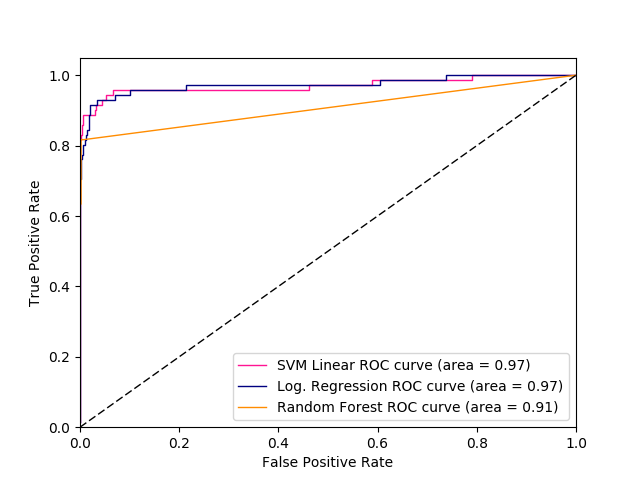
\includegraphics[width=0.7\textwidth]{figures/roc_auc_brazilian_travel_related}
  \label{fig:roc_curve}
\end{figure}

After the selection of our classification model, we decided to classify all the Portuguese dataset and draw some statistics from the results. The trained Linear SVM classifier was used to predict whether tweets were travel-related or not, since it was the model presenting the best score under the F1-score metric (as shown in Table~\ref{classifiers}). From a total of 7.8M tweets, our classifier was able identified 37,300 travel-related entries.

Fig.~\ref{predicted} depicts the distribution of travel-related tweets over the days of the week. We can see that the first three business days (Monday, Tuesday and Wednesday) are the ones on which the Twitter activity is higher for both cities in our study.

\begin{figure}[!htbp]
  \caption{Positive Predicted Tweets per Day of Week}
  \centering
    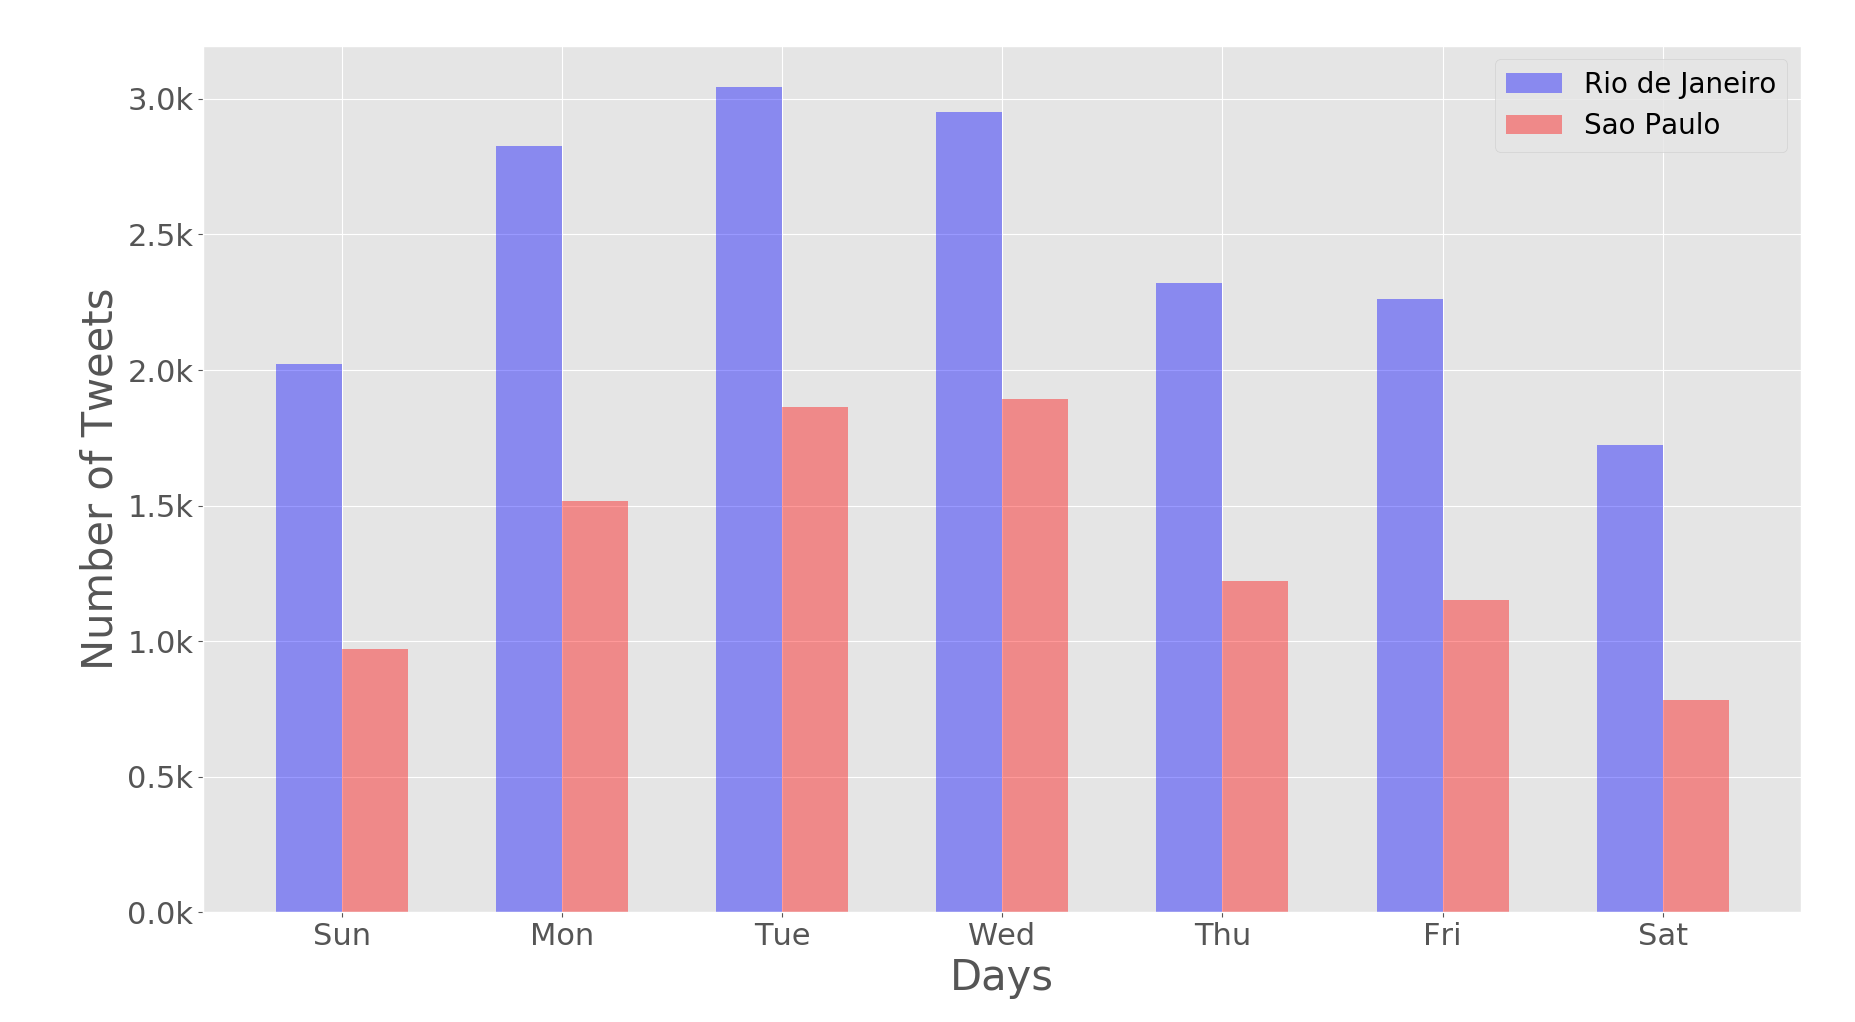
\includegraphics[width=0.7\textwidth]{figures/predicted_day_of_week}
    \label{predicted}
\end{figure}

\begin{figure}[!htbp]
  \caption{Rio de Janeiro Heatmap to the positive tweets}
  \centering
    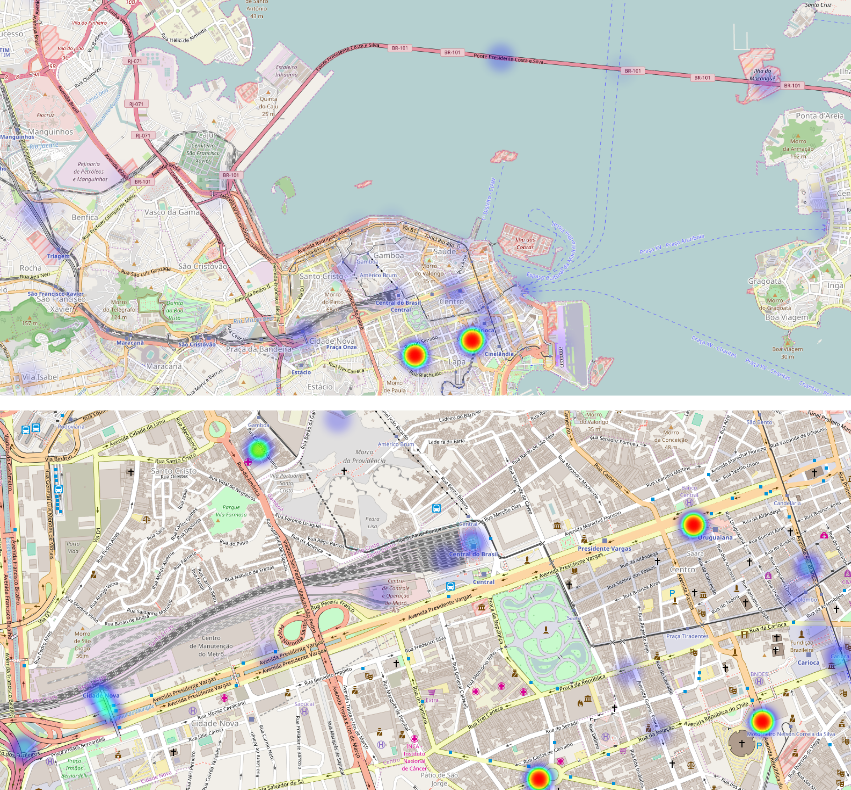
\includegraphics[width=0.725\textwidth]{figures/rio_1}
    \label{rio_heatmap}
\end{figure}

\begin{figure}[h]
  \caption{São Paulo Heatmap to the positive tweets}
  \centering
    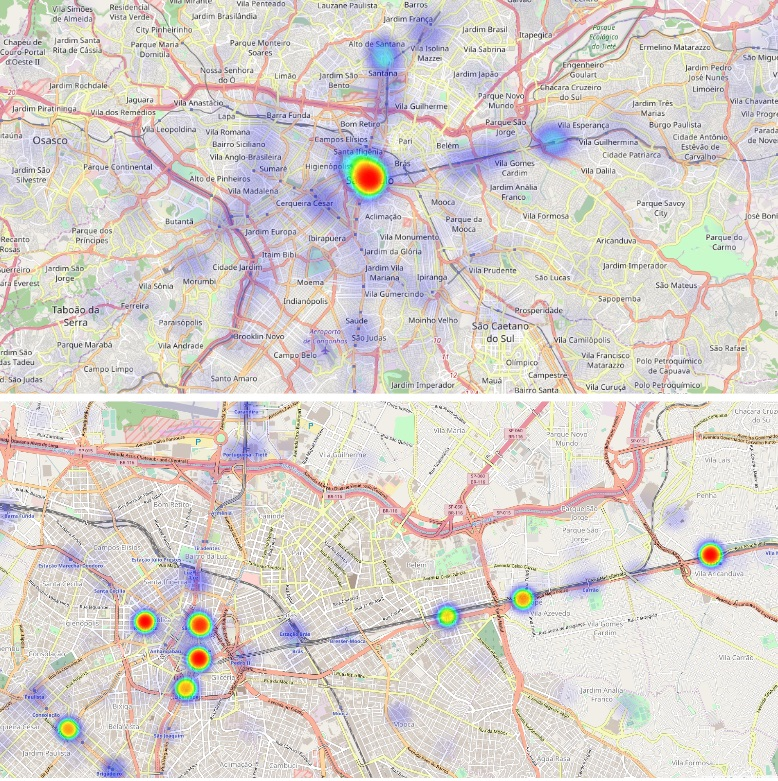
\includegraphics[width=0.725\textwidth]{figures/sp_1}
    \label{sp_heatmap}
\end{figure}

In order to understand the spatial distribution of travel-related tweets we generated a heatmap for both cities. From the heatmap of RJ, illustrated in Fig.~\ref{rio_heatmap}, it is possible to identify that some agglomerations of tweets are located at Central do Brasil, Cidade Nova and Triagem train stations, as well as at Uruguaiana, Maracanã and Carioca metro stations. The Rio-Niterói bridge, connecting Rio de Janeiro to Niterói, as well as the piers on both sides also presented considerable clouds of tweets classified as travel-related.

The heatmap for the city of SP, illustrated in Fig.~\ref{sp_heatmap}, was also an interesting case to observe. Almost every agglomeration matched some metro or train station. Estação Brás, Tatuapé, Belém, Estação Paulista, Sé, Liberdade were some of the stations highlighted in the heatmap. We could also identify a little agglomeration of travel-related tweets at Congonhas airport, even though no tweets seemed to mention the word \textit{plane} explicitly in the training of our classification model.

\subsection{Final Remarks}
The experiment previous described explores an approach of supervised learning using as training examples a set of manually annotated tweets extracted from the whole datasets with the support of a term-based regular expression. The overall methodology is concerned with the problem of construct a fine-grained Twitter training set for the travel domain and also the automatic identification of travel-related tweets from a large scale corpus. We combined different word representations to verify whether our classification model could learn relations between words at both syntactic and semantic levels. After using standard techniques such as bag-of-words and bag-of-embeddings, we have used them combined yielding results that showed that these different groups of features can complement each other, with respect to Portuguese-speaking tweets.

\section{English Travel-related Classification}

Similar to the experiment of Portuguese travel-related classification, we built a model to discriminate english-speaking travel-related tweets. However, by following the same approach, final results were not improved with the combination of two different groups of features, bag-of-words and bag-of-embeddings.

The overall experiment steps as well as the final results are showed in the following subsections.

\subsection{Data Collection and Preparation}
Differently from the Portuguese experiment, tweets were collected from New York City during a period of two months, between days March 12 and May 12, 2017. Ignoring all non-English tweets the resulting dataset comprehends 4M tweets.

Regarding the preparation of data, we used the same preprocessing operations for each tweet present in our dataset:

\begin{itemize}
	\item \textbf{Lowercasing:} The message was converted to lowercase;
	\item \textbf{Transforming repeated characters:} Sequences of characters repeated more than three times were transformed, e.g. "sooooo" was converted to "sooo";
	\item \textbf{Cleaning:} Removing URLs and user mentions.
\end{itemize}

\subsection{Features Selection}
The features groups used in this experiments were the same presented in Section~\ref{subsec:features_4_3_2}.

\subsection{Training and Test Datasets}

The construction of the training and test sets were supported by the same term-based approach used in Section~\ref{subsec:training_test_datasets_portuguese} in order to filter tweets from the whole collection, i.e. we used the regular expression $space + term + space$ with each term presented in Table~\ref{tab:terms}. Firstly, 1,686 tweets were selected for each of both cases, travel-related and non-related. The travel-related set was strictly balanced in order to have almost the same amount of examples for each of the travel-modes involved in this study. The non-related training set is composed of several subjects that are not related to travel, e.g. football, leisure, politician, personal tweets, among others.

\subsection{Classification}
We choose a supervised learning approach in order to provide a robust solution for the classification task. Three learning algorithms were selected to conduct our experiments, namely Support Vector Machines (SVM), Logistic Regression (LR) and Random Forests (RF). The SVM classifier was tested under the \textit{linear} kernel function. To the LR classifier, standard parameters were applied, whereas the RF classifier was defined with 100 trees in the forest. The \textit{gini criterion} and the maximum number of features were limited to those previous mentioned in Section~\ref{subsec:features_4_3_2}, in the case of the RF classifier.
The performance of the resulting models will be compared in terms of \emph{precision}, \emph{recall} and the \emph{F1-score}.

\subsection{Preliminary Results}\label{subsec:preliminar_results}
In our first attempt, 10-fold cross-validation was applied for each model using, independently, bag-of-words and bag-of-embeddings as features. Results
showed us that all the models obtained good performance regarding the selected evaluation metrics. The best model in this experiment was the Random Forests classifier trained with bag-of-words features, performing an F1-score of 0,977. Indeed, all the models that used bag-of-words features, in particular, revealed high scores as can be observed in Table~\ref{tab:first_experiment}. This may be explained by the similar vocabulary present in both training and test sets. One important note is that all travel-mode classes are known by the model before the classification of the test set. This may not be true in real-world scenarios. Although the results presented in Table~\ref{tab:first_experiment}, we tried to combine both features and conclude that, contrarily to the Portuguese travel-related experiment, the performance was decreased when comparing it with the one obtained from the usage BoW features in the experiment. To further investigate the robustness of the best features group we designed another experiment that is explained in Section~\ref{subsec:leave_one_group_out}.

\begin{table}[htbp]
	\small
	\centering
	\caption{Preliminary Results}
	\label{tab:first_experiment}
	\begin{tabular}{|c|c|c|c|c|}
		\hline
		\textbf{Classifier} & \textbf{Features} & \textbf{Precision} & \textbf{Recall}  & \textbf{F1-score} \\ \hline
		\multirow{2}{*}{\textbf{Linear SVM}} & BoE (200) & 0,90883   & 0,83634 & 0,87089  \\
		& \textbf{BoW} & \textbf{0,96298}   & \textbf{0,97652} & \textbf{0,96962}  \\ \hline
		\multirow{2}{*}{\textbf{Logistic Regression}} & BoE (100) & 0,90172   & 0,84948 & 0,87447  \\
		& \textbf{BoW} & \textbf{0,96431}   & \textbf{0,98042} & \textbf{0,97222}  \\ \hline
		\multirow{2}{*}{\textbf{Random Forests}} & BoE (100) & 0,81283   & 0,83600 & 0,82394  \\
		& \textbf{BoW} & \textbf{0,96569}   & \textbf{0,98997} & \textbf{0,97764}  \\ \hline
	\end{tabular}
\end{table}

\subsection{\emph{Leave-one-group-out}}\label{subsec:leave_one_group_out}
The second experiment follows a \emph{leave-one-group-out} strategy. Meaning that one travel-mode class if left out of the training set and moved into the test set. This way, the behaviour of the learned model when facing a completely unknown travel-mode class can be evaluated.
A model for each hidden mode of transport class was built, and evaluation is carried as the previous experiment. The datasets composition of each experiment led in this strategy can be observed in Table~\ref{tab:leave}.

\begin{table}[htbp]
	\small
	\centering
	\caption{Datasets Composition}
	\label{tab:leave}
	\begin{tabular}{|c|c|c|c|c|}
		\hline
		\multirow{2}{*}{\textbf{\begin{tabular}[c]{@{}c@{}}Travel-Mode \\ Class\end{tabular}}} & \multicolumn{2}{c|}{\textbf{Training Set}} & \multicolumn{2}{c|}{\textbf{Test Set}} \\ \cline{2-5} & \textbf{Pos.} & \textbf{Neg.} & \textbf{Pos.}  & \textbf{Neg.}  \\ \hline
		Taxi & 1,372 & \multirow{6}{*}{1,686}   & 314 & \multirow{6}{*}{300}  \\
		Train & 1,369 & & 317 & \\
		Car  & 1,369 & & 317 & \\
		Bike & 1,386 & & 300 & \\
		Walk & 1,469 & & 217 & \\
		Bus  & 1,375 & & 311 & \\ \hline
	\end{tabular}
\end{table}

Each learning model experiment was made varying the hidden travel-mode class, which is unknown for our classifier in the training process. This method was performed in order to evaluate the sensitivity and robustness of the models built in our first experiment, described in Section~\ref{subsec:preliminar_results}. Table~\ref{tab:results} presents the best results for each model, as so its features and tuning parameters. The results from the models using bag-of-embeddings features revealed a consistent performance, i.e. they do not change even with the variation of the size of the feature vectors.

According to results, all classification models have performed reasonably well under the bag-of-embeddings features group, although the dimensionality used being different for the Linear SVM classifier.

\begin{table}[htbp]
	\small
	\centering
	\caption{\emph{Leave one group out} experiments results for SVM, LR and RF classifiers}
	\label{tab:results}
	\begin{tabular}{|c|c|c|c|c|}
		\hline
		\textbf{Classifier} & \textbf{Features}  & \textbf{Precision} & \textbf{Recall}  & \textbf{F1-score} \\ \hline
		\multirow{2}{*}{\textbf{Random Forests}} & BoW & 0,40774 & 0,07474 & 0,12629  \\
		& \textbf{BoE (50)}  & \textbf{0,80278} & \textbf{0,76194} & \textbf{0,78447}  \\ \hline
		\multirow{2}{*}{\textbf{Logistic Regression}} & BoW & 0,40774 & 0,07474 & 0,12629  \\
		& \textbf{BoE (50)}  & \textbf{0,84882} & \textbf{0,75702} & \textbf{0,80219}  \\ \hline
		\multirow{2}{*}{\textbf{Linear SVM}} & BoW & 0,41527 & 0,07153 & 0,12203  \\
		& \textbf{BoE (200)} & \textbf{0,86374} & \textbf{0,75715} & \textbf{0,81289}  \\ \hline
	\end{tabular}
\end{table}

\begin{figure}[htbp]
	\centering
	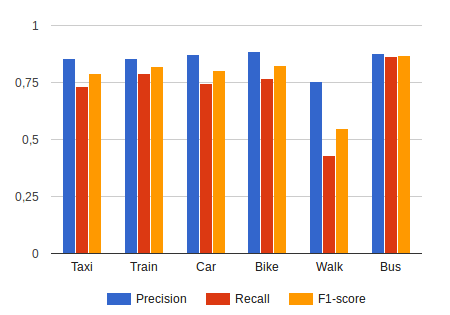
\includegraphics[scale=0.7]{figures/svm_linear_leave_one_out_emb_200.png}
	\caption{SVM model with BoE(200) for each travel mode}
	\label{fig:svm_leave}
\end{figure}

After testing each model with a hidden travel-mode class, the models trained with bag-of-words features demonstrated poor performance when facing unknown travel-modes, revealing higher sensitivity and lower generalization capabilities in comparison to the bag-of-embeddings version. The generalization power is an important and crucial characteristic for our desired solution. In a real world scenario is very likely that we will face a higher variety of categories that were not taken into consideration in the training phase of our model.

\begin{table}[htbp]
	\centering
	\small
	\caption{Sample of tweet messages correctly classified}
	\label{tab:tweets_examples}
	\resizebox{\textwidth}{!}{\begin{tabular}{|c|}
		\hline
		when you get into your uber and he has a pipe in the back \\
		a ground stop for \#ewr is no longer in effect \#flightdelay \\
		snowy walk to work. \#blizzard2017 \#centralpark \#noreaster2017 \@ bethesda terrace fountain -  \textbf{Figure~\ref{fig:central_park}} \\
		m.t.a. n.y.c subways: w train irregular subway service at whitehall street-south ferry \#traffic - \textbf{Figure~\ref{fig:brooklyn}} \\ \hline
	\end{tabular}}
\end{table}

The best result of the \emph{leave-one-group-out} was the Linear SVM model, with the dimensionality of 200 in the size of the feature vectors. Figure~\ref{fig:svm_leave} presents the results of each experiment led for the different hidden travel-mode classes. An interesting point to observe is the low performance obtained to the experiment with the travel-mode class "Walk" hidden. This is due to the different semantic and syntactic contexts that the word \emph{walk} is used. Although all other classes can be used in the same context, for example, \emph{car}, \emph{train}, or \emph{bus}, usually the word \emph{walk} is not applied in the same way.

Having the experiments concluded, we used the best model, in this case, Linear SVM for the dimensionality of 200, to predict the 4M tweets that composed the NYC dataset. Almost 300,000 tweets were classified as travel-related. After the classification step, a sample of 10,000 tweets was taken from all the travel-related classified tweets and it was produced a heat-map distribution in order to verify which are the most concentrated zones. Such distribution enables the identification of associations with metro, train, bus stations. In Figure~\ref{fig:brooklyn}, that shows the south of the Manhattan island and also the Brooklyn bridge, it is possible no note some agglomerations over the bridge and also in the port and closed to the Wall Street(4.5) where there are some metro stations. The Central Park is one place that also took our attention since presented several agglomerations of tweets. In this particular place, tweets related to the walk class were correctly identified.

\begin{figure}[htbp]
	\centering
	\begin{subfigure}[htbp]{0.8\textwidth}
		\centering
		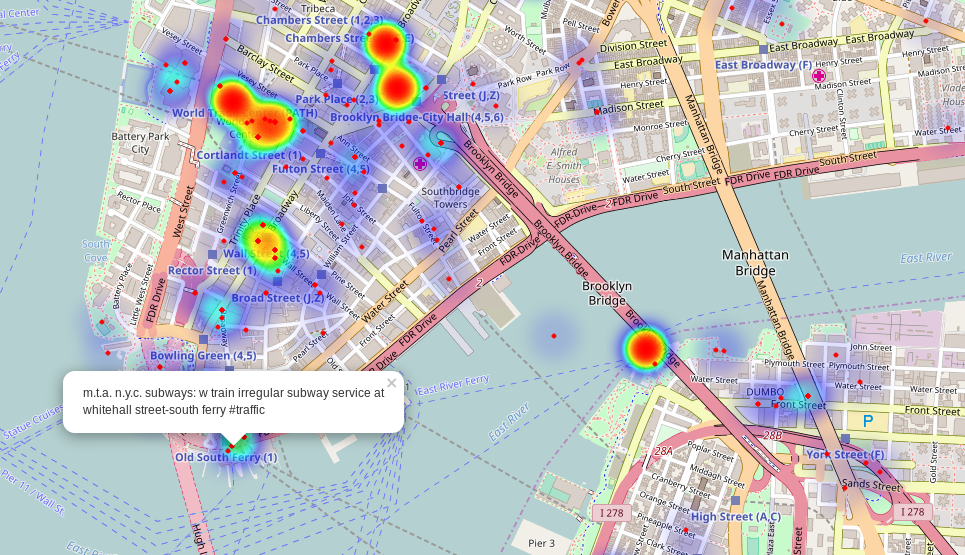
\includegraphics[width=0.9\columnwidth]{figures/nyc_map.png}
		\caption{}
		\label{fig:brooklyn}
	\end{subfigure}
	
	\medskip
	
	\centering
	\begin{subfigure}[htbp]{0.8\textwidth}
		\centering
		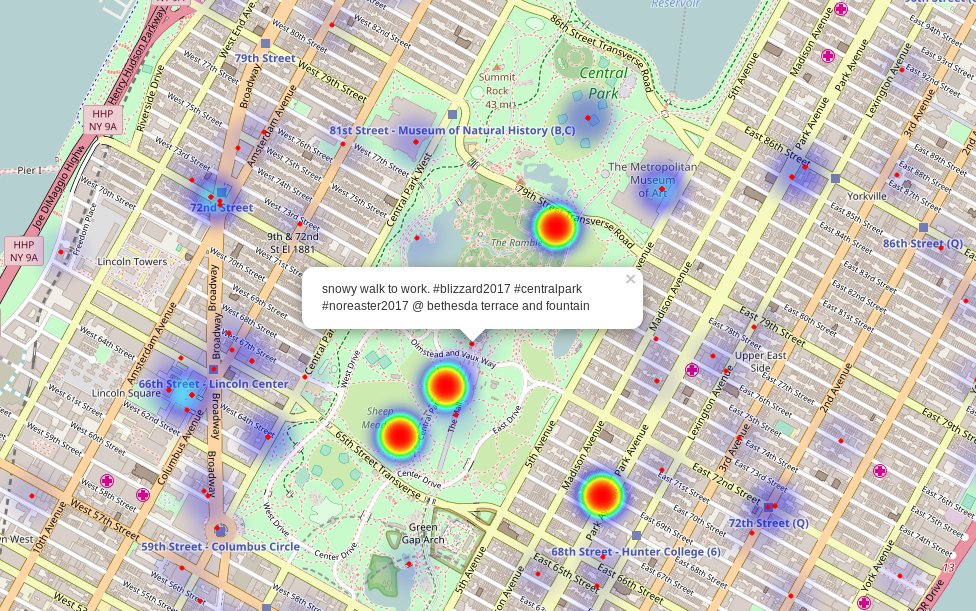
\includegraphics[width=0.9\columnwidth]{figures/nyc_map2.png}
		\caption{}
		\label{fig:central_park}
	\end{subfigure}
	
	\caption[Spatial density of the predicted tweets]{Spatial density of the travel-related predicted tweets in New York City: (a) South of Manhattan and over the Brooklyn Bridge, (b) Central Park}
	\label{fig:nyc__geographical_distribution}
\end{figure}

\subsection{Concluding Remarks}
The main objective of this experiment was to devise a travel-related tweet classifier using word embeddings trained with geo-located English-speaking tweets. Similar to the Portuguese travel-related classification, we tried to build our model using a combined approach relying on bag-of-words and bag-of-embeddings features; however, results presented signs of dependency in the bag-of-words features and the performance have also decreased. By looking in the results of the best group, bag-of-words, we doubt about the existence of overfitting, and so, a \emph{leave-one-group-out} strategy was applied to attempt reproduce and validate the results obtained from classification models in preliminary experiment. Such an strategy shows that our training and test sets were very similar to each other. In this second experiment, we excluded one of the travel-modes classes, which resulted in the fact that models using bag-of-words features could not maintain the performance previously demonstrated. Comparatively to the approach based on bag-of-words, the models using bag-of-embeddings features revealed consistency, robustness, and effectiveness in the classification task. The Linear SVM model proved to be the best option with respect to the performance metrics considered in this work. We thus used that model trained with bag-of-embeddings to predict all the English tweets from our NYC dataset, whose results showed significant improvement over a standard bag-of-words baseline. Finally, we applied the resulting classifier to a stream of geo-located tweets in New York City, which was able to depict important spatio-temporal patterns.

\section{Topic Modelling}\label{sec:topic_modeling}
This section is related to the experiment of automatically characterize tweets in two different Brazilian cities, Rio de Janeiro and São Paulo. We used an unsupervised learning approach to tackle the task of topic modelling in order to compare both cities and see if there are differences between subjects people talked about. Automatic characterization of text messages is a laborious and time consuming task since it is necessary to assure the right level of abstraction in the learning model; very much similarly to human minds, which essentially present a bounded rationality nature, our learning model needs to be trained in order to assimilate the necessary knowledge and perform the appropriate analogies so as to discover different topics within the tweets' contents. The premises to implement such a mechanism are presented and discussed in the following subsections.

\subsection{Data Selection}
The data selected to conduct this experiment is correspondent to a period of two months, between days March 12 and May 12, 2017. 

The resulting datasets sum up a total of 12.5M and 6.3M tweets for Rio de Janeiro and for São Paulo, respectively. Due to the problem detected in Section~\ref{sec:data_collection}, we filtered the data in order to only use the tweets that were actually inside the cities' areas. The final composition of the datasets is presented in Table~\ref{tab:datasets}, and the results of the filtering process shown that almost 6M tweets were not located inside the bounding-boxes of the cities.

\begin{table*}[ht]
	\small
	\centering
	\caption{Datasets composition}
	\label{tab:datasets}
	\resizebox{\textwidth}{!}{\begin{tabular}{|c|c|c|c|c|c|c|}
		\hline
		\textbf{City}  & \textbf{All} & \textbf{PT} & \textbf{Non-PT} & \textbf{\begin{tabular}[c]{@{}c@{}}In \\ Bounding-Box\end{tabular}} & \textbf{\begin{tabular}[c]{@{}c@{}}Out\\ Bounding-Box\end{tabular}} & \textbf{\begin{tabular}[c]{@{}c@{}}PT and \\ In Bounding-Box\end{tabular}} \\ \hline
		Rio de Janeiro & 12,531,000 & 10,570,000 & 1,961,000 & 8,644,000 & 3,886,000 & 7,353,000 \\ \hline
		São Paulo & 6,352,000 & 4,886,000 & 1,466,000 & 4,247,000 & 2,105,000 & 3,313,000 \\ \hline
	\end{tabular}}
\end{table*}
	
The subset of data composed by Portuguese tweets and located inside the cities' bounding-boxes was used to conduct the experiment described in this section. Such subset can be sum up to a total of 7.3M and 3.3M for Rio de Janeiro and São Paulo, respectively.

\subsection{Data Preparation}
Usually, to tackle topic modelling tasks in text documents it is required several pre-processing steps. Such pre-processing to the data helps the operations made by the LDA model, which is the technique used here. Removing unnecessary words, transforming words into their root form as so deleting all the punctuation are some of the common text mining pre-processing steps. Here, each tweet of both datasets was submitted to a required group of pre-processing operations in order to train a LDA model and proceed with the experiments. The pre-processing steps were the ones detailed below.

\begin{itemize}
	\item \textbf{Lowercasing:} Every message presented in a tweet was converted into lower case;
	\item \textbf{Cleaning Entities and Numbers:} Removing \textit{URLs}, user mentions, \textit{hashtags} and digits from the text message;
	\item \textbf{Lemmatization:} Only plural words were transformed into singular ones;
	\item \textbf{Transforming repeated characters:} Sequences of characters repeated more than three times were transformed, e.g. "loooool" was converted to "loool";
	\item \textbf{Punctuation Removal:} Every punctuation was removed as well as smiles (e.g. \texttt{:)}, \texttt{:-)}, \texttt{=D}) or even \emph{emoticons};
	\item \textbf{Stop Words Removal:} The removing of this kind of words was made using the Portuguese NLTK dictionary;
	\item \textbf{Short Tokens Removal:} Words such as 'kkk', 'aaa', 'aff' and other of the same style were removed.
\end{itemize}

After the data preparation phase, 772,017 tweets have their message empty which conclude that its content was irrelevant for the final experiment phase.

\subsection{Features Selection}
Topic modelling requires, like in other learning model, a group of features to be trained. In this case, we used the Bag-of-Words representation matrix - which is a representation where each document is converted to a frequency vector according to the number of occurrences of each word in the message. The set of features was limit to a dictionary containing 10,000 words and it only took into account uni-grams in the message content. The dictionary was also limited to words that occur in a maximum percentage of 40$\%$ in the whole dataset, avoiding common words that were not removed because they were not included in the NLTK Stop Words list. The minimal occurrence value for a word being considered was set to 10.

\subsection{LDA Model Parametrization}
In order to understand and see the LDA model performance, we set five different numbers for the topics results parameter of the training process: 5, 10, 20, 25 and 50 topics, being this the one with better results. The number of iterations to train the model was set to 20, since our desired was to reproduce the experiment made by G. Lansley et al.~\cite{lansley2016geography} to the city of London. Finally but not the least, each tweet in the datasets was treated as a single document comprehending that, in total, 6,580,983 different documents were used in the model training process. The complete pipeline according to all the steps taken to conduct this experiment is observable in Figure~\ref{fig:pipeline_lda}.

\iffalse
\begin{figure}[h]
	\centering
	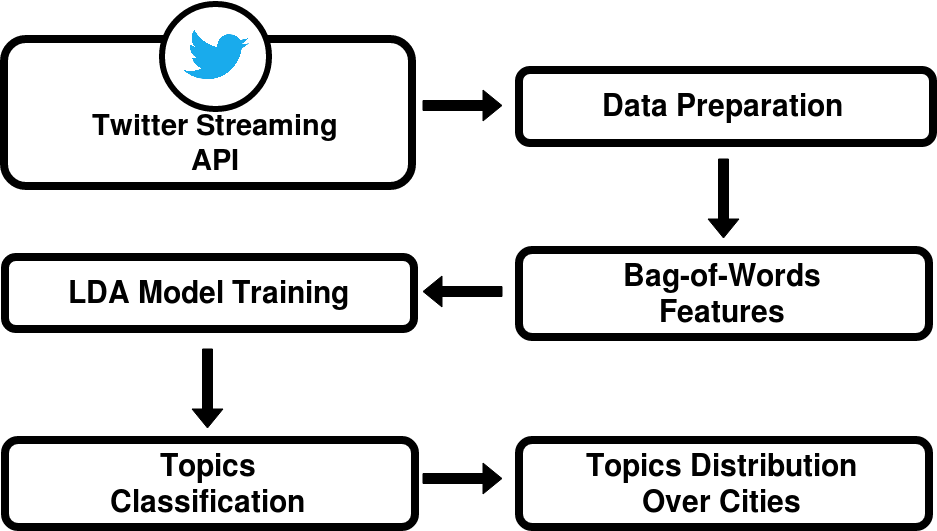
\includegraphics[width=0.6\linewidth]{figures/pipeline_lda.png}
	\caption{Correspondent pipeline of the topic modelling experiment}
	\label{fig:pipeline_lda}
\end{figure}
\fi

\subsection{Results and Analysis}
To evaluate the experimental results obtained for each model (where the difference underlies on the variation of the number of topics), a list with the most frequent 50 words for each topic was extracted. In Table~\ref{tab:topics_classification} we can observe a sample (20 top words) selected out of the 50 studied. Nonetheless, the final evaluation took into consideration all the  50 outputted words.
	
\begin{table}[h]
	\centering
	\caption{Example of the topics classification}
	\label{tab:topics_classification}
	\resizebox{\textwidth}{!}{\begin{tabular}{c|c}
			\hline
			\textbf{\begin{tabular}[c]{@{}c@{}}Words\\ (only 20 words)\end{tabular}} & \textbf{\begin{tabular}[c]{@{}c@{}}Topic\\ Classification\end{tabular}} \\ \hline
			\begin{tabular}[c]{@{}c@{}}paulo, vai, hoje, dia, jogo, ser, melhor, time, vamo, brazil, \\ todo, santo, brasil, gol, cara, aqui, agora, corinthiam, ano, palmeiro, vem, ...\end{tabular} & \begin{tabular}[c]{@{}c@{}}Sports and\\ Games\end{tabular} \\ \hline
			\begin{tabular}[c]{@{}c@{}}vou, dia, dormir, queria, hoje, ficar, casa, semano, quero, ter, \\ ainda, hora, agora, sono, aula, acordar, acordei, cedo, fazer, prova, ...\end{tabular} & \begin{tabular}[c]{@{}c@{}}Wake-up\\ Messages\end{tabular} \\ \hline
			\begin{tabular}[c]{@{}c@{}}top, social, artist, vote, the, award, army, bom, voting, doi, \\ bogo, oitenta, sipda, today, vinte, prepara, cypher, oito, quatro, man, ...\end{tabular} & \begin{tabular}[c]{@{}c@{}}Voting and\\ Numbers\end{tabular} \\ \hline
			\begin{tabular}[c]{@{}c@{}}marco, nada, falar, emilly, gente, quer, nao, pessoa, nunca, fala, \\ vai, falando, sobre, chama, agora, manda, vem, mensagem, vivian, bbb, ...\end{tabular} & \begin{tabular}[c]{@{}c@{}}Big Brother\\ Brazil 2017\end{tabular} \\ \hline
			\begin{tabular}[c]{@{}c@{}}paulo, brazil, sao, santo, vila, just, parque, posted, photo, shopping, \\ paulista, centro, bernardo, jardim, cidade, avenido, praia, santa, campo, academia\end{tabular} & \begin{tabular}[c]{@{}c@{}}Tourism and\\ Places\end{tabular} \\ \hline
		\end{tabular}}
\end{table}

We also selected and manually analyse a random sample (with the size of 200) of tweets for each topic. This sampling was done in order to get better consistency and trustiness about the classification and characterization of the tweets.

It was found a group of 50 topics which had the largest number of distinct topics between them. However, there were topics which theme was the same (e.g. Love and Romance Problems or Brazilian Football \textit{versus} European Football). Within this, such groups were aggregate into the same topic, \textit{Relationships} and \textit{Sports and Games}, respectively. After this grouping process, a total of 29 different topics was achieved. 

Some tweets that have added complexity to our classification objective, such as, for example, "\textit{queria namorar um mano parecido com o josh}" (Relationship) and "\textit{como eu queria meus amigos aqui agora cmg}" (Friendship), raised some doubts about which topic this tweets may belong: Relationship, Friendship or even Actions or Intentions. In a perspective of context, the first tweet belongs to the theme \texttt{flirt}, which is directly related to Relationship. The theme on the second tweet is missing the company of friends, i.e. conviviality, which is related to Friendship. The decision of join the two topics was due to the proximity between them which have as content both types of tweets, talking about love/relationship and friendship, and with this in consideration both topics should be aggregated in order to assure the desired consistency in the classification.

The final set of topics (50 topics) to be considered was selected accordantly to the most recurring subjects. The final classification and details associated with the whole dataset for each city is presented in Table~\ref{tab:final_classification}. Almost every topics demonstrated a balanced distribution, with exception of \textit{Relationships and Friendship} and \textit{Personal Feelings} for Rio de Janeiro and São Paulo, respectively. The difference that appear in this topics is a consequence of the final grouping process, since there was a considerable number of words been shared among this topics. This issue complicated our classification task, compelling to an high amount of undesired aggregations.

\begin{table}[ht]
	\small
	\caption{Final results of the LDA topics aggregation}
	\label{tab:final_classification}
	\resizebox{\textwidth}{!}{\begin{tabular}{l|cc|cc|c}
		\hline
		\multicolumn{1}{c|}{\multirow{2}{*}{\textbf{Topic Group}}} & \multicolumn{2}{c|}{\textbf{Rio de Janeiro}} & \multicolumn{2}{c|}{\textbf{São Paulo}} & \multicolumn{1}{c|}{\multirow{2}{*}{\textbf{Diff (\%)}}} \\ \cline{2-5}
		\multicolumn{1}{c|}{} & \textbf{No. Tweets} & \textbf{Percentage (\%)} & \textbf{No. Tweets} & \textbf{Percentage (\%)} & \multicolumn{1}{c|}{} \\ \hline
		Academic Activities & 101,590 & 1,54\% & 90,616 & 3,30\% & -1,76\% \\
		Actions or Intentions & 600,030 & 9,12\% & 128,710 & 4,69\% & \textbf{+4,43\%} \\
		Antecipation and Socialising & 132,606 & 2,01\% & 0 & 0,00\% & \textbf{+2,01\%} \\
		BBB17 & 122,054 & 1,85\% & 68,385 & 2,49\% & -0,64\% \\
		Body, Appearances and Clothes & 160,342 & 2,44\% & 71,447 & 2,60\% & -0,17\% \\
		Food and Drink & 167,204 & 2,54\% & 58,407 & 2,13\% & +0,41\% \\
		Health & 119,013 & 1,81\% & 0 & 0,00\% & \textbf{+1,81\%} \\
		Holidays and Weekends & 104,695 & 1,59\% & 79,610 & 2,90\% & -1,31\% \\
		Informal Conversations & 272,502 & 4,14\% & 138,848 & 5,06\% & -0,92\% \\
		Live Shows, Social Events and Nightlife & 359,342 & 5,46\% & 140,240 & 5,11\% & +0,35\% \\
		Mood & 139,287 & 2,12\% & 138,399 & 5,04\% & \textbf{-2,92\%} \\
		Movies and TV & 285,198 & 4,33\% & 39,778 & 1,45\% & \textbf{+2,89\%} \\
		Music and Artists & 84,407 & 1,28\% & 78,142 & 2,85\% & 1,56\% \\
		Negativism, Pessimism and Anger & 229,104 & 3,48\% & 183,050 & 6,67\% & \textbf{-3,18\%} \\
		Numbers, Quantities and Classification & 86,897 & 1,32\% & 78,160 & 2,85\% & -1,53\% \\
		Optimism and Positivism & 106,714 & 1,62\% & 39,725 & 1,45\% & +0,18\% \\
		Personal Fellings & 375,735 & 5,71\% & 532,331 & 19,38\% & \textbf{-13,67\%} \\
		Politics & 81,254 & 1,23\% & 46,758 & 1,70\% & 0,47\% \\
		Relationships and Friendship & 1,524,804 & 23,17\% & 187,541 & 6,83\% & \textbf{+16,34\%} \\
		Religion & 183,174 & 2,78\% & 66,788 & 2,43\% & +0,35\% \\
		Routine Activities & 334,216 & 5,08\% & 82,421 & 3,00\% & +2,08\% \\
		Slang and Profinities & 241,676 & 3,67\% & 44,620 & 1,62\% & +2,05\% \\
		Social Media Applications & 105,809 & 1,61\% & 44,073 & 1,60\% & +0,01\% \\
		Sport and Games & 382,479 & 5,81\% & 133,047 & 4,84\% & +0,97\% \\
		Tourism and Places & 59,288 & 0,90\% & 86,519 & 3,15\% & -2,25\% \\
		Transportation and Travel & 130,261 & 1,98\% & 63,923 & 2,33\% & -0,35\% \\
		Weather & 91,302 & 1,39\% & 42,588 & 1,55\% & -0,16\% \\
		Shopping & 0 & 0,00\% & 44,470 & 1,62\% & \textbf{-1,62\%} \\
		Voting & 0 & 0,00\% & 37,687 & 1,37\% & \textbf{-1,37\%} \\ \hline
	\end{tabular}}
\end{table}
	
Additionally to the manual verification of a sample of tweets for each topic, we also produced a temporal week day distribution,  with the objective to observe if some topics had more mentions in certain days than others.

For making such observations some assumptions were made in relation with some \textit{hot} topics. More specifically, we think that is valid to assume that people will talk more about \textit{Religion} in the weekend, since they go to the church in those days. The same result is likely to happen for topics like \textit{Holidays and Weekends} or \textit{Sports and Games}, since events related to this thematics occur during specific time-frames. 

Only 12 topics of the finals 29 were selected for this part of the study, predicting them and comparing the final results, such as, but not limited to, \textit{Sports and Games}, \textit{Religion}, \textit{Holidays and Weekends}, \textit{Movies and TV}, \textit{Live Shows, Social Events and Nightlife}. The temporal distribution is showed in Figure~\ref{fig:topics_heat_maps} as a heat map, where each row is independent from the others.

The necessity of applying such restrictions is due to the need of seeing in which days each topic is more talked about. For both cities the topic \textit{Sports and Games} is more mentioned in Tuesdays and Saturdays. Indeed, this observation correlates with the days that topic-related events happens. Namely, Tuesdays and Wednesday correspond to the days when the \textit{UEFA Champions League} competition happens and Saturdays and Sundays to the days of \textit{Brazilian Football League} games. \textit{Holidays and Weekends} was a topic with interesting results regarding the temporal distribution, presenting Sundays as the day where more people talk about it. 

Furthermore, it is worth mentioning that our model had successfully discover a topic related to Big Brother Brazil 2017 (BBB17), a well-known reality show. The amount of geo-located tweets concerning this topic was considerable (1.85\% and 2.49\%, in RJ and SP, respectively), rising the question about what led people to geo-located them in such topic.
	
\begin{figure}[h]
	\centering
	\begin{subfigure}{0.49\textwidth}
		\centering
		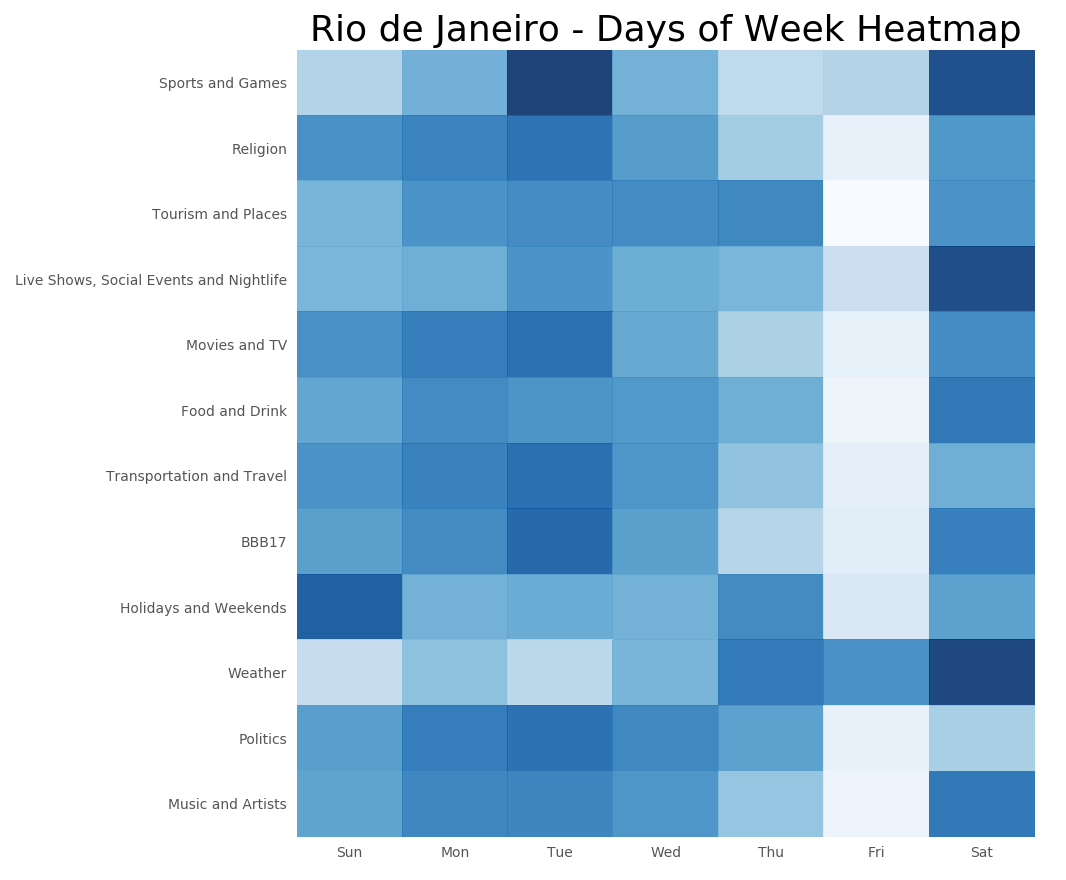
\includegraphics[width=1.0\linewidth]{figures/rio_topics_heatmap.png}
		\label{fig:rio}
	\end{subfigure}
	\begin{subfigure}{0.49\textwidth}
		\centering
		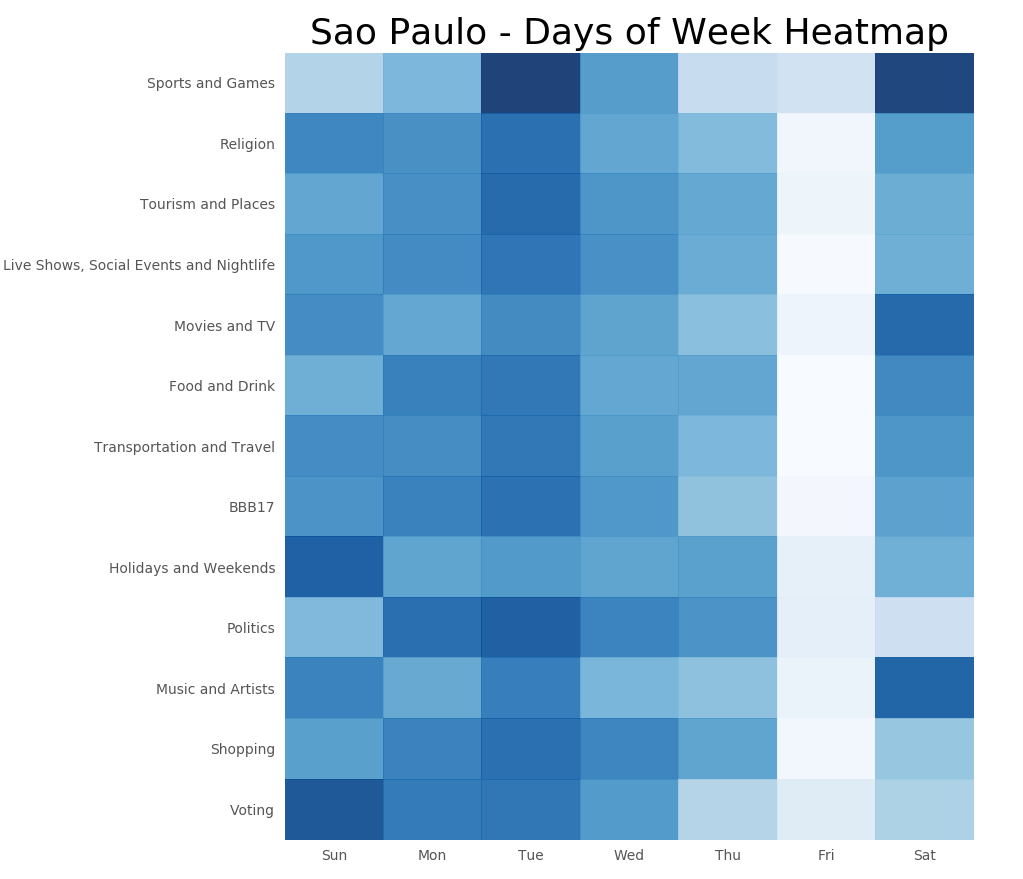
\includegraphics[width=1.0\linewidth]{figures/sp_topics_heatmap.png}
		\label{fig:sp}
	\end{subfigure}
	\caption[Day-of-the-week Twitter activity]{Day-of-the-week activity per each topic in both cities, Rio de Janeiro and São Paulo}
	\label{fig:topics_heat_maps}
\end{figure}
	
\subsection{Final Remarks}
The methodology reported across this experiment is concerned with topic modelling over two datasets from two Brazilian cities in order to characterize the topics that people talked about and compare the results in both scenarios. LDA models usually requires documents of large size, or at least more complex than a single tweet, in order to get good performance. A traditional approach was followed considering each tweet as a document instead of trying aggregate tweets in more complex documents taking into consideration some criteria, e.g. grouping by date and hour. The final results showed that topics in both cities are very similar and only two of them are unique. With exception of topics - \textit{Relationships and Friendship} and \textit{Personal Feelings}, the percentage difference between similar topics was comprehended in the interval 0.16-4.43\% evidencing the fact that both cities are similar besides the different factors that characterize each one: population, culture, lifestyle and also the region where the city is located in. Although all this analysis, we can not assure that inside a topic we do not have more topics hidden. Our classification was limited to the verification of the 50 top words and the manually verification of a sample of 200 tweets since the resulting amount of tweets for each topic is impossible to verify one by one. Due to this, another classification approach need to be explored and a promising one was proposed by D. Ramage et al.~\cite{ramage2010characterizing}. The classification will be automatic by adding a supervised extra layer to the pipeline. However, to assure trustiness in the results the data may be manually labelled for the training phase of the model classification or, at least, have reliable sources, for example, exploring the topics provide by the Wikipedia articles\footnote{\url{https://dumps.wikimedia.org/ptwiki/20170601/}}.


\section{Summary}
This chapter has the purpose of report the experiments conduct over this dissertation period in order to help the implementation of the different modules designed in our framework architecture.

Firstly, two different classification models for travel-related tweets were developed taking into consideration two possible languages in texts, Portuguese and English. Under the implementation of the Portuguese classification, we were able to prove that the combination of conventional techniques (bag-of-words) and recent ones (word embeddings) performed very well. However, for the English classification, the high performance values obtained using only bag-of-words led us to suspect of the existence of overfitting in the examples used as training. An \textit{leave-one-group-out} strategy was taken to proved such phenomenon and conclude our suspicions of similar words being shared in training and test datasets. When a transport-class was omited, the model with bag-of-words performed worst than the one using only bag-of-embeddings. For this reason we were obligated to the application of two different classification models in the development of the frameworks' travel-related classification module. This allows consistency and robustness in the classification of tweets for two distinct speaking languages.

Moreover, topic modelling techniques were applied under Portuguese-speaking tweets for two different \textit{megacities}, Rio de Janeiro and São Paulo, in order to extract information that may enabling interesting characterizations in different regions/zones of the cities regarding temporal and geographical distributions. Although huge restrictions regardind the labelling of each topic, results show promising contributions and informations to the \textit{smart cities} entities, allowing until this point possible identifications of what are the most \textit{hot} topics in each region.